\documentclass[tikz]{standalone}
\usepackage{amsmath}
\usepackage{amssymb}
\usepackage{amsfonts}
\usepackage{tikz}
\usetikzlibrary {arrows.meta} 

\thispagestyle{empty}
\begin{document}

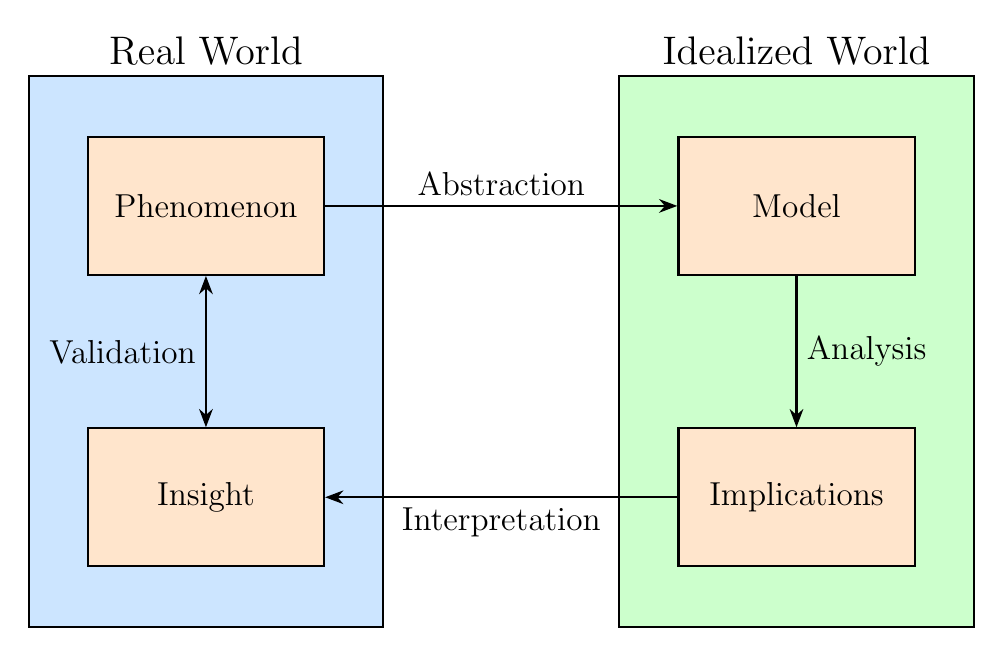
\begin{tikzpicture}[thick, >=Stealth]

\definecolor{softred}{RGB}{255, 204, 204}
\definecolor{softorange}{RGB}{255, 229, 204}
\definecolor{softyellow}{RGB}{255, 255, 204}
\definecolor{softgreen}{RGB}{204, 255, 204}
\definecolor{softblue}{RGB}{204, 229, 255}
\definecolor{softpurple}{RGB}{230, 190, 220}

% Big rectangles
\node[draw, fill=softblue, minimum width=4.5cm, minimum height=7cm, label=above:{\Large Real World}] (realworld) at (0, 0) {};
\node[draw, fill=softgreen, minimum width=4.5cm, minimum height=7cm, label=above:{\Large Idealized World}] (abstractworld) at (7.5, 0) {};  % Abstract World

% Boxes inside Real World
\node[draw, fill=softorange, minimum width=3cm, minimum height=1.75cm, align=center] (phenomenon) at (0, 1.85) {\large Phenomenon};
\node[draw, fill=softorange, minimum width=3cm, minimum height=1.75cm, align=center] (validation) at (0, -1.85) {\large Insight};

% Boxes inside Abstract World
\node[draw, fill=softorange, minimum width=3cm, minimum height=1.75cm, align=center] (model) at (7.5, 1.85) {\large Model};
\node[draw, fill=softorange, minimum width=3cm, minimum height=1.75cm, align=center] (results) at (7.5, -1.85) {\large Implications};  % Implications

% Arrows between boxes
\draw[->] (phenomenon.east) -- node[above]{\large Abstraction} (model.west);
\draw[->] (model.south) -- node[right]{\large Analysis} (results.north);
\draw[->] (results.west) -- node[below]{\large Interpretation} (validation.east);
\draw[<->] (validation.north) -- node[left]{\large Validation} (phenomenon.south);

\end{tikzpicture}
\end{document}
